%!TEX root = main.tex
%TODO Figure 4: trajectories are not continuous because of snipping them. That's why a red traj is red and outside the collision area.

\section{Recurrent Neural Network: Binary classification} \label{sec:rnn_clf}

We first briefly describe RNNs and LSTMs, as these were not covered in homework assignments.
Then, we analyze the performance of an LSTM for the same binary classification as before, and compare with the SVM implementation.

\subsection{Introduction}

Recurrent Neural Networks (RNNs) have been shown to extract sequential information and generate highly complex sequences as documents, translations, music and more.
In comparison to n-gram models, which have been used in language model for speech recognition, a RNN makes a prediction by a high-dimensional interpolation between training samples.
N-gram models predict by creating a distribution, based on the number of exact matches between the recent history and the training set (graves). 

\begin{figure}
	\centering
	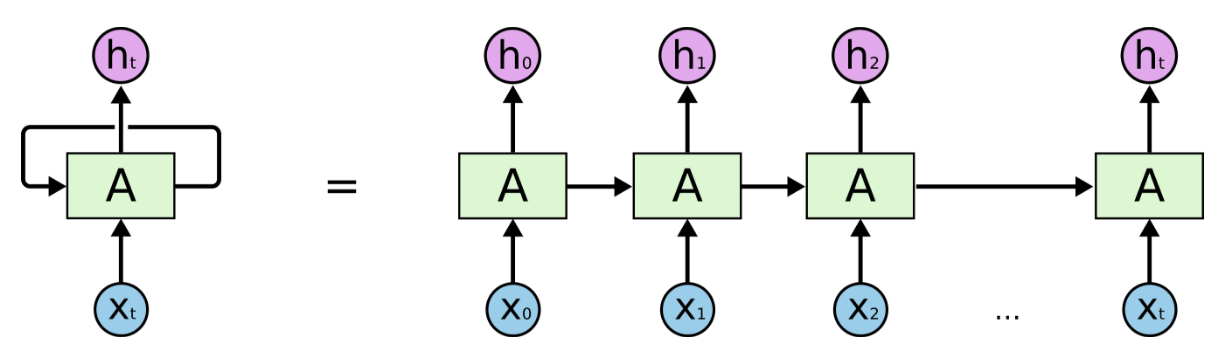
\includegraphics [trim=0 0 0 0, clip, angle=0, width=0.8\columnwidth,
	keepaspectratio]{figures/rnn_unrolled}
	\caption{Illustration of a RNN in it's enrolled (left) and unrolled (right) form. Each sequential input $x_t$ is fed in at timestep $t$, transformed by the activation cell $A$ and output and fed into the next cell as hidden state $h_t$. (colah)} 
	\label{fig:rnn_unrolled} 
\end{figure}

In theory RNNs can be trained by backpropagating the error along the chain of cells.
However, every step involves a multiplication with the weight matrix $W$, which, in many cases, results in either an exploding or vanishing gradient (see class exercise).
The exploding/vanishing gradient problem is, in practice, addressed by gradient clipping (cs232 lecture).
\meXX{are these 2 diff methods to address vanishing gradient problem?}The $\textit{vanishing gradient problem}$ is leveraged by a specific architecture of RNNs, called $\textit{Long Short-term Memory}$ (LSTM) networks.
LSTMs split up the RNN's hidden state into a hidden and a cell state.
The cell state, similar to in ResNets, is updated by a sum-operation, rather than a whole transformation \meXX{unclear}(SEE FIGURE ... for the comparison of RNN to LSTM cell).
The gradient along a sum-operation splits up equally and thereby allows to propagate until the beginning of the sequence without vanishing.\meXX{unclear}

\begin{figure}
	\centering
	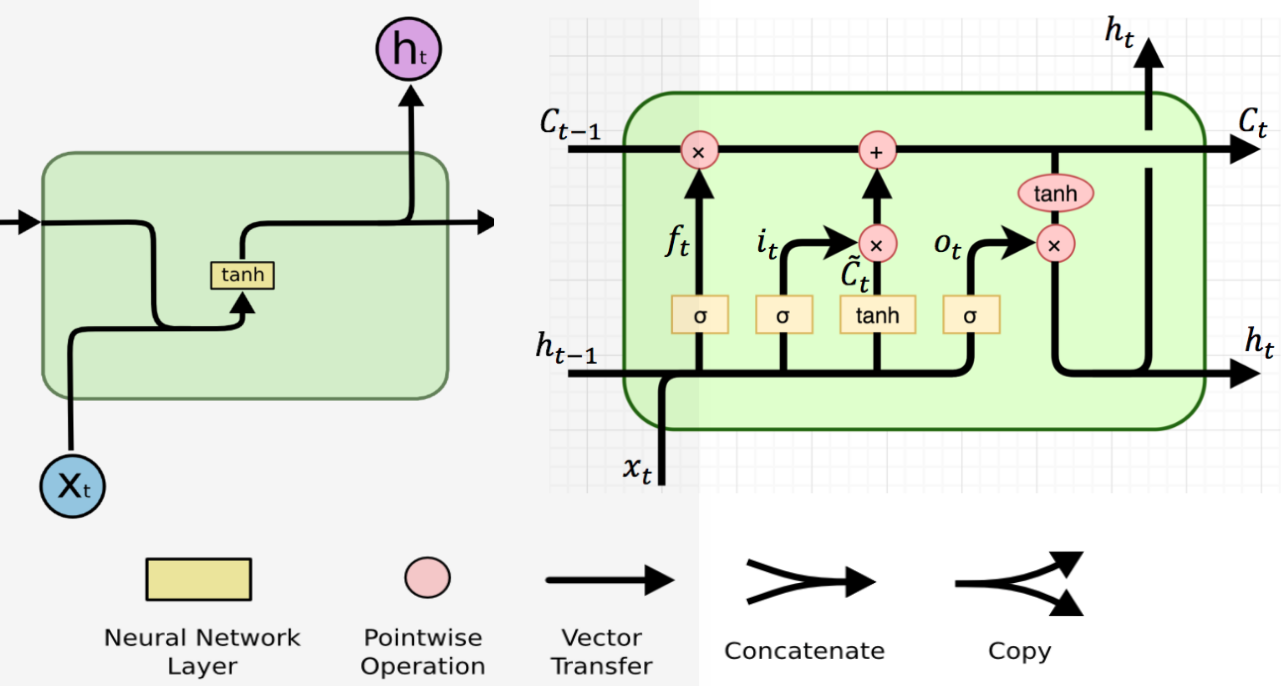
\includegraphics [trim=0 0 0 0, clip, angle=0, width=1.0\columnwidth,
	keepaspectratio]{figures/rnn_lstm}
	\caption{Activation cell of a traditional RNN (top) and a LSTM (bottom). LSTM propagates the cell $c_t$ and hidden $h_t$ state. With ignoring the forget gate $f_t$, $c_t$ is only updated by sum operations. The gradient along a sum-operation splits up equally and thereby allows to propagate until the beginning of the sequence without vanishing. ResNets have introduced a similar change in the CNN architecture (resnet paper). (changhau)} 
	\label{fig:rnn_lstm} 
\end{figure}

%TODO take graph of graves paper.
The LSTM is computed according to the following composite function\meXX{add citation} (graves):
\begin{equation}
\begin{aligned}
& i_t = \sigma(W_{xi}x_t + W_{hi}h_{t-1} + W_{ci}c_{t-1} + b_i)\\
& f_t = \sigma(W_{xf}x_t + W_{hf}h_{t-1} + W_{cf}c_{t-1} + b_f)\\
& c_t = f_tc_{t-1} + i_ttanh(W_{xc}x_t + W_{hc}h_{t-1} + b_c)\\
& o_t = \sigma(W_{xo}x_t + W_{ho}h_{t-1} + W_{co}c_{t-1} + b_o)\\
& h_t = o_ttanh(c_t)
\end{aligned}
\label{eq:lstm_eq} 
\end{equation}
where $\sigma$ is the sigmoid function, $i_t$, $f_t$, $o_t$ and $c_t$ are the input gate, forget gate, output gate and cell activation vectors.
All weight matrices have the same meaning, for example $W_{hf}$ is the hidden-forget weight matrix.\meXX{same meaning?}
For clarity, bias terms are omitted\meXX{from what?}.
Figuratively speaking, the input gate regulates how much information is taken from the new input $x_t$.
The forget gate can erase the cell memory and thereby controls the duration of time dependency during sequence prediction.
The cell state is the part of memory that propogates between hidden nodes.
The output gate regulates how much information from the hidden cell state is propagated into the output hidden state.

\subsection{LSTMs for binary classification}
We used LSTM networks for the same binary classification task from~\cref{sec:svm}.
LSTMs are able to extract the sequential information more naturally than SVM, so we expected to see better classification accuracy in the train and test datasets.
We used Python and the $\textit{Tensorflow}$ library to implement the LSTMs.

Again, the full trajectories have been precompiled into snippets of static sequence length $T$.
At each time step, the input vector is the relative pedestrian position at time $t$: $x_t \in \Re^{1x2}$.
For binary classification, we use a many-to-one architecture.
The output is calculated at the output layer by using a logistic sigmoid for binary classification:
\begin{equation}
y_t = \sigma(W_{hout}h_t + b_out)
\label{eq:bin_class_out} 
\end{equation}
where $y_t \in [0,1]$, $W_{hout} \in \Re^{n_{hidden} \text{x} 1}$, and $n_{hidden}$ is the number of hidden units.
The weight matrices and biases are initialized with random noise $\sim\mathcal{N}(0,1)$.
We use the least mean squared error (LMSE) loss function.
The network is optimized by a stochastic gradient descent (SGD) method with the goal to minimize the loss over the weight matrices and their biases.

\subsection{Hyperparameters}
Again, there are many hyperparameters to optimize, including the number of hidden units, batch size, learning rate, and number of training epochs.
It is very time intensive to search over all hyperparamters.
We briefly summarize the hyperparameters' effects on performance, using validation accuracy as the performance metric.
The output of our full grid search is in our posted code (file: rnn\_classifier\_hyperparameters.txt).

The best hyperparameters were batch size of 5, $n_{hidden}=256$, $T=10$, and 3 training epochs, and we used a learning rate of 0.001.

Performance generally levels off after 3-5 training epochs.
For large T, more hidden units are required to handle the higher dimension of the input data.
Specifically, when $T>10$, $n_{hidden}=8$ got $<50\%$ accuracy, but performance improved with $n_{hidden}=64$ (we ranged T from 2-50, and $n_{hidden}$ from 8-256).
Small batch size tended to improve the performance, but it was not a clear trend (we ranged batch size from 1-10).

We also investigate the effect of training set size on performance in~\cref{fig:svm_num_datapts}.
The blue line corresponds to the LSTM classifier, which is not greatly affected by training set size (close to 80\% throughout).
The LSTM classifier is not as sensitive as SVM to training set size. 

\subsection{Results}
After optimizing hyperparameters and confirming we have a sufficient amount of training data, we trained the LSTM binary classifier.
The overall test accuracy was 80.4\%.

\cref{fig:svm_labels} \& \cref{fig:rnn_labels} look pretty similar.
Both classifiers learned about the ``cross zone'', perform relatively well on data that is predicted to be class 0, and struggle with false negatives far from the vehicle.
The fact that both classifiers indicates that type of data is especially challenging to classify correctly.

\begin{figure}
\centering
\begin{subfigure}{.25\textwidth}
  \centering
  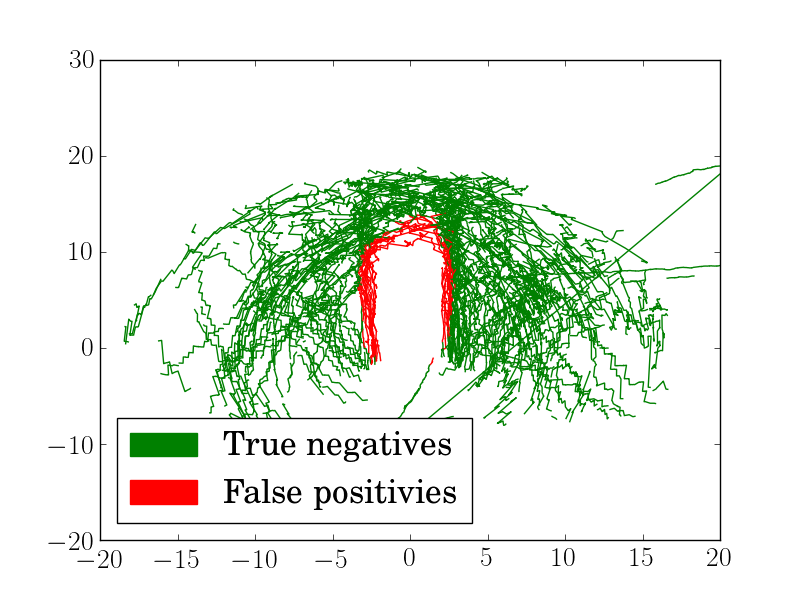
\includegraphics[width=.9\linewidth]{figures/rnn_label0}
  \caption{Trajs. labeled ``No Cross''}
  \label{fig:rnn_label0}
\end{subfigure}%
\begin{subfigure}{.25\textwidth}
  \centering
  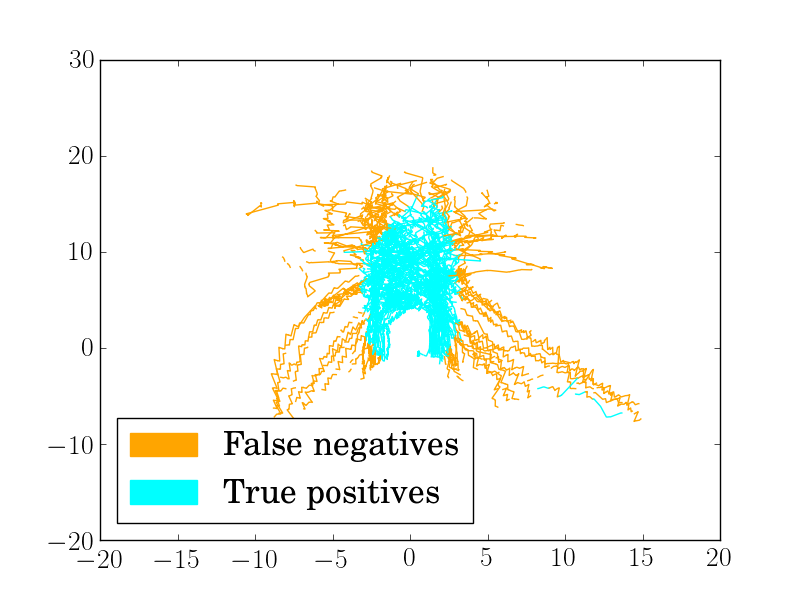
\includegraphics[width=.9\linewidth]{figures/rnn_label1}
  \caption{Trajs. labeled ``Cross''}
  \label{fig:rnn_label1}
\end{subfigure}
\caption{Predicted labels on test set with LSTM classifier. On the left, trajectory snippets that were predicted label 0 (green is correct, red is incorrect). On the right, trajectory snippets that were predicted label 1 (cyan correct, orange incorrect). Across the whole test set, 80\% accuracy was achieved. Compare with~\cref{fig:svm_labels}}
\label{fig:rnn_labels}
\end{figure}
